\section{mr::point\_\-base$<$ C, T $>$ Struct Template Reference}
\label{structmr_1_1point__base}\index{mr::point_base@{mr::point\_\-base}}
{\tt \#include $<$mr\-Vector.h$>$}

Inheritance diagram for mr::point\_\-base$<$ C, T $>$::\begin{figure}[H]
\begin{center}
\leavevmode
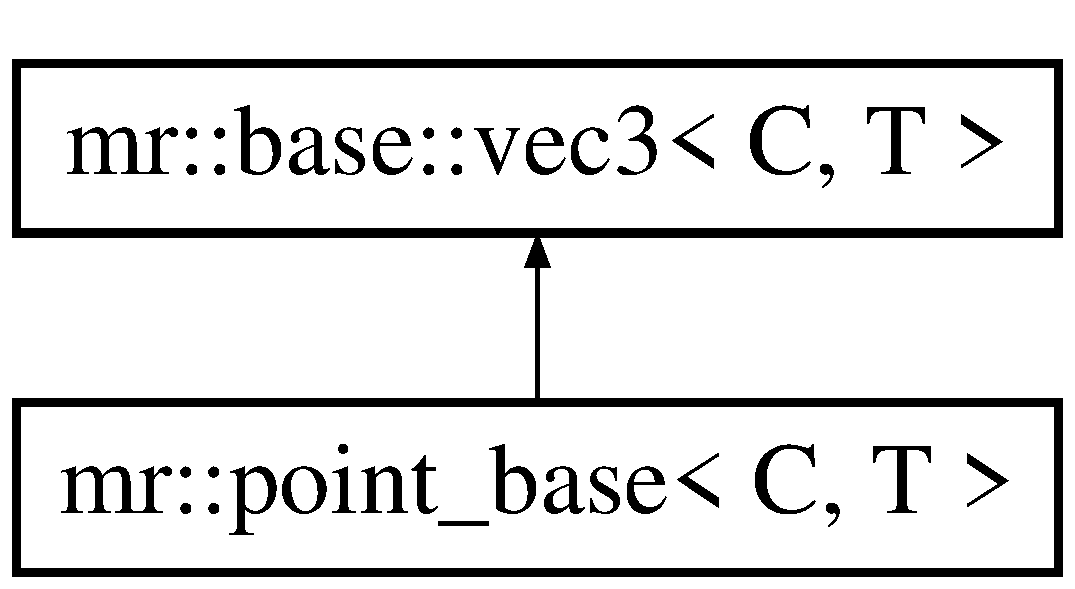
\includegraphics[height=2cm]{structmr_1_1point__base}
\end{center}
\end{figure}
\subsection*{Public Types}
\begin{CompactItemize}
\item 
typedef {\bf point\_\-base}$<$ C, T $>$ {\bf self}
\end{CompactItemize}
\subsection*{Public Member Functions}
\begin{Indent}{\bf Space Conversions}\par
\begin{CompactItemize}
\item 
void {\bf to\-Object} (const mi\-State $\ast$const state)
\item 
void {\bf to\-World} (const mi\-State $\ast$const state)
\item 
void {\bf to\-Camera} (const mi\-State $\ast$const state)
\item 
void {\bf to\-Screen} (const mi\-State $\ast$const state)
\item 
void {\bf to\-NDC} (const mi\-State $\ast$const state)
\item 
void {\bf to\-Raster} (const mi\-State $\ast$const state)
\item 
void {\bf to\-Light} (const mi\-State $\ast$const state)
\item 
void {\bf from\-Object} (const mi\-State $\ast$const state)
\item 
void {\bf from\-World} (const mi\-State $\ast$const state)
\item 
void {\bf from\-Camera} (const mi\-State $\ast$const state)
\item 
void {\bf from\-Screen} (const mi\-State $\ast$const state)
\item 
void {\bf from\-NDC} (const mi\-State $\ast$const state)
\item 
void {\bf from\-Raster} (const mi\-State $\ast$const state)
\item 
void {\bf from\-Light} (const mi\-State $\ast$const state)
\item 
void {\bf to} (const mi\-State $\ast$const state, const {\bf space::type} to\-Space)
\item 
void {\bf from} (const mi\-State $\ast$const state, const {\bf space::type} from\-Space)
\item 
void {\bf transform} (const mi\-State $\ast$const state, const {\bf space::type} from\-Space, const {\bf space::type} to\-Space)
\end{CompactItemize}
\end{Indent}
\begin{Indent}{\bf Constructors}\par
\begin{CompactItemize}
\item 
{\bf point\_\-base} ()
\begin{CompactList}\small\item\em Default constructor. \item\end{CompactList}\item 
{\bf point\_\-base} (const T xx, const T yy=0.0f, const T zz=0.0f)
\begin{CompactList}\small\item\em Multielement constructors. \item\end{CompactList}\item 
{\bf point\_\-base} (const mi\-State $\ast$const state, const {\bf space::type} to\-Space, const T xx, const T yy, const T zz)
\item 
{\bf point\_\-base} (const mi\-State $\ast$const state, const {\bf space::type} from\-Space, const C \&v)
\item 
template$<$class X, class Y, class Oper$>$ {\bf point\_\-base} (const {\bf base::exp}$<$ X, Y, Oper $>$ \&e)
\begin{CompactList}\small\item\em Single element constructors. \item\end{CompactList}\item 
{\bf point\_\-base} ({\bf k\-No\-Construct})
\item 
{\bf point\_\-base} (const C \&b)
\item 
{\bf point\_\-base} (const T b)
\end{CompactItemize}
\end{Indent}
\begin{Indent}{\bf Copy constructor}\par
\begin{CompactItemize}
\item 
{\bf point\_\-base} (const {\bf self} \&b)
\end{CompactItemize}
\end{Indent}
\begin{Indent}{\bf Assignment}\par
\begin{CompactItemize}
\item 
template$<$class X, class Y, class Oper$>$ const {\bf self} \& {\bf operator=} (const {\bf base::exp}$<$ X, Y, Oper $>$ \&e)
\begin{CompactList}\small\item\em Handle assignment when we deal with a chained operation. \item\end{CompactList}\item 
const {\bf self} \& {\bf operator=} (const {\bf self} \&b)
\begin{CompactList}\small\item\em Assignment of similar object. \item\end{CompactList}\item 
const {\bf self} \& {\bf operator=} (const C \&b)
\begin{CompactList}\small\item\em Assignemnt of base class object. \item\end{CompactList}\item 
const {\bf self} \& {\bf operator=} (const T b)
\begin{CompactList}\small\item\em Assignment of base type. \item\end{CompactList}\end{CompactItemize}
\end{Indent}
\begin{Indent}{\bf REFERENCE OPERATORS (MODIFY IN PLACE)}\par
\begin{CompactItemize}
\item 
const {\bf self} \& {\bf operator $\ast$=} (const T b)
\item 
const {\bf self} \& {\bf operator $\ast$=} (const C \&b)
\item 
const {\bf self} \& {\bf operator $\ast$=} (const mi\-Matrix a)
\item 
{\bf self} {\bf operator $\ast$} (const mi\-Matrix m) const 
\begin{CompactList}\small\item\em Matrix post-multiplication. \item\end{CompactList}\item 
const {\bf self} \& {\bf operator $\ast$=} (const {\bf matrix} \&m)
\begin{CompactList}\small\item\em In-place matrix post-multiplication. \item\end{CompactList}\item 
{\bf self} {\bf operator $\ast$} (const {\bf matrix} \&m) const 
\begin{CompactList}\small\item\em Matrix post-multiplication. \item\end{CompactList}\end{CompactItemize}
\end{Indent}
\subsection*{Static Public Attributes}
\begin{CompactItemize}
\item 
{\bf point\_\-base}$<$ C, T $>$ {\bf k\-Origin}
\end{CompactItemize}
\subsubsection*{template$<$class C, typename T$>$ struct mr::point\_\-base$<$ C, T $>$}



\subsection{Member Typedef Documentation}
\index{mr::point_base@{mr::point\_\-base}!self@{self}}
\index{self@{self}!mr::point_base@{mr::point\_\-base}}
\subsubsection{\setlength{\rightskip}{0pt plus 5cm}template$<$class C, typename T$>$ typedef {\bf point\_\-base}$<$ C, T $>$ {\bf mr::point\_\-base}$<$ C, T $>$::{\bf self}}\label{structmr_1_1point__base_w0}




Reimplemented from {\bf mr::base::vec3$<$ C, T $>$} {\rm (p.\,\pageref{structmr_1_1base_1_1vec3_w0})}.

\subsection{Constructor \& Destructor Documentation}
\index{mr::point_base@{mr::point\_\-base}!point_base@{point\_\-base}}
\index{point_base@{point\_\-base}!mr::point_base@{mr::point\_\-base}}
\subsubsection{\setlength{\rightskip}{0pt plus 5cm}template$<$class C, typename T$>$ {\bf mr::point\_\-base}$<$ C, T $>$::{\bf point\_\-base} ()\hspace{0.3cm}{\tt  [inline]}}\label{structmr_1_1point__base_z75_0}


Default constructor. 

\index{mr::point_base@{mr::point\_\-base}!point_base@{point\_\-base}}
\index{point_base@{point\_\-base}!mr::point_base@{mr::point\_\-base}}
\subsubsection{\setlength{\rightskip}{0pt plus 5cm}template$<$class C, typename T$>$ {\bf mr::point\_\-base}$<$ C, T $>$::{\bf point\_\-base} (const T {\em xx}, const T {\em yy} = 0.0f, const T {\em zz} = 0.0f)\hspace{0.3cm}{\tt  [inline]}}\label{structmr_1_1point__base_z75_1}


Multielement constructors. 

\index{mr::point_base@{mr::point\_\-base}!point_base@{point\_\-base}}
\index{point_base@{point\_\-base}!mr::point_base@{mr::point\_\-base}}
\subsubsection{\setlength{\rightskip}{0pt plus 5cm}template$<$class C, typename T$>$ {\bf mr::point\_\-base}$<$ C, T $>$::{\bf point\_\-base} (const mi\-State $\ast$const {\em state}, const {\bf space::type} {\em to\-Space}, const T {\em xx}, const T {\em yy}, const T {\em zz})\hspace{0.3cm}{\tt  [inline]}}\label{structmr_1_1point__base_z75_2}


\index{mr::point_base@{mr::point\_\-base}!point_base@{point\_\-base}}
\index{point_base@{point\_\-base}!mr::point_base@{mr::point\_\-base}}
\subsubsection{\setlength{\rightskip}{0pt plus 5cm}template$<$class C, typename T$>$ {\bf mr::point\_\-base}$<$ C, T $>$::{\bf point\_\-base} (const mi\-State $\ast$const {\em state}, const {\bf space::type} {\em from\-Space}, const C \& {\em v})\hspace{0.3cm}{\tt  [inline]}}\label{structmr_1_1point__base_z75_3}


\index{mr::point_base@{mr::point\_\-base}!point_base@{point\_\-base}}
\index{point_base@{point\_\-base}!mr::point_base@{mr::point\_\-base}}
\subsubsection{\setlength{\rightskip}{0pt plus 5cm}template$<$class C, typename T$>$ template$<$class X, class Y, class Oper$>$ {\bf mr::point\_\-base}$<$ C, T $>$::{\bf point\_\-base} (const {\bf base::exp}$<$ X, Y, Oper $>$ \& {\em e})\hspace{0.3cm}{\tt  [inline]}}\label{structmr_1_1point__base_z75_4}


Single element constructors. 

\index{mr::point_base@{mr::point\_\-base}!point_base@{point\_\-base}}
\index{point_base@{point\_\-base}!mr::point_base@{mr::point\_\-base}}
\subsubsection{\setlength{\rightskip}{0pt plus 5cm}template$<$class C, typename T$>$ {\bf mr::point\_\-base}$<$ C, T $>$::{\bf point\_\-base} ({\bf k\-No\-Construct})\hspace{0.3cm}{\tt  [inline]}}\label{structmr_1_1point__base_z75_5}


\index{mr::point_base@{mr::point\_\-base}!point_base@{point\_\-base}}
\index{point_base@{point\_\-base}!mr::point_base@{mr::point\_\-base}}
\subsubsection{\setlength{\rightskip}{0pt plus 5cm}template$<$class C, typename T$>$ {\bf mr::point\_\-base}$<$ C, T $>$::{\bf point\_\-base} (const C \& {\em b})\hspace{0.3cm}{\tt  [inline]}}\label{structmr_1_1point__base_z75_6}


\index{mr::point_base@{mr::point\_\-base}!point_base@{point\_\-base}}
\index{point_base@{point\_\-base}!mr::point_base@{mr::point\_\-base}}
\subsubsection{\setlength{\rightskip}{0pt plus 5cm}template$<$class C, typename T$>$ {\bf mr::point\_\-base}$<$ C, T $>$::{\bf point\_\-base} (const T {\em b})\hspace{0.3cm}{\tt  [inline]}}\label{structmr_1_1point__base_z75_7}


\index{mr::point_base@{mr::point\_\-base}!point_base@{point\_\-base}}
\index{point_base@{point\_\-base}!mr::point_base@{mr::point\_\-base}}
\subsubsection{\setlength{\rightskip}{0pt plus 5cm}template$<$class C, typename T$>$ {\bf mr::point\_\-base}$<$ C, T $>$::{\bf point\_\-base} (const {\bf self} \& {\em b})\hspace{0.3cm}{\tt  [inline]}}\label{structmr_1_1point__base_z76_0}




\subsection{Member Function Documentation}
\index{mr::point_base@{mr::point\_\-base}!from@{from}}
\index{from@{from}!mr::point_base@{mr::point\_\-base}}
\subsubsection{\setlength{\rightskip}{0pt plus 5cm}template$<$class C, typename T$>$ void {\bf mr::point\_\-base}$<$ C, T $>$::from (const mi\-State $\ast$const {\em state}, const {\bf space::type} {\em from\-Space})\hspace{0.3cm}{\tt  [inline]}}\label{structmr_1_1point__base_z74_15}


\index{mr::point_base@{mr::point\_\-base}!fromCamera@{fromCamera}}
\index{fromCamera@{fromCamera}!mr::point_base@{mr::point\_\-base}}
\subsubsection{\setlength{\rightskip}{0pt plus 5cm}template$<$class C, typename T$>$ void {\bf mr::point\_\-base}$<$ C, T $>$::from\-Camera (const mi\-State $\ast$const {\em state})\hspace{0.3cm}{\tt  [inline]}}\label{structmr_1_1point__base_z74_9}


\index{mr::point_base@{mr::point\_\-base}!fromLight@{fromLight}}
\index{fromLight@{fromLight}!mr::point_base@{mr::point\_\-base}}
\subsubsection{\setlength{\rightskip}{0pt plus 5cm}template$<$class C, typename T$>$ void {\bf mr::point\_\-base}$<$ C, T $>$::from\-Light (const mi\-State $\ast$const {\em state})\hspace{0.3cm}{\tt  [inline]}}\label{structmr_1_1point__base_z74_13}


\index{mr::point_base@{mr::point\_\-base}!fromNDC@{fromNDC}}
\index{fromNDC@{fromNDC}!mr::point_base@{mr::point\_\-base}}
\subsubsection{\setlength{\rightskip}{0pt plus 5cm}template$<$class C, typename T$>$ void {\bf mr::point\_\-base}$<$ C, T $>$::from\-NDC (const mi\-State $\ast$const {\em state})\hspace{0.3cm}{\tt  [inline]}}\label{structmr_1_1point__base_z74_11}


\index{mr::point_base@{mr::point\_\-base}!fromObject@{fromObject}}
\index{fromObject@{fromObject}!mr::point_base@{mr::point\_\-base}}
\subsubsection{\setlength{\rightskip}{0pt plus 5cm}template$<$class C, typename T$>$ void {\bf mr::point\_\-base}$<$ C, T $>$::from\-Object (const mi\-State $\ast$const {\em state})\hspace{0.3cm}{\tt  [inline]}}\label{structmr_1_1point__base_z74_7}


\index{mr::point_base@{mr::point\_\-base}!fromRaster@{fromRaster}}
\index{fromRaster@{fromRaster}!mr::point_base@{mr::point\_\-base}}
\subsubsection{\setlength{\rightskip}{0pt plus 5cm}template$<$class C, typename T$>$ void {\bf mr::point\_\-base}$<$ C, T $>$::from\-Raster (const mi\-State $\ast$const {\em state})\hspace{0.3cm}{\tt  [inline]}}\label{structmr_1_1point__base_z74_12}


\index{mr::point_base@{mr::point\_\-base}!fromScreen@{fromScreen}}
\index{fromScreen@{fromScreen}!mr::point_base@{mr::point\_\-base}}
\subsubsection{\setlength{\rightskip}{0pt plus 5cm}template$<$class C, typename T$>$ void {\bf mr::point\_\-base}$<$ C, T $>$::from\-Screen (const mi\-State $\ast$const {\em state})\hspace{0.3cm}{\tt  [inline]}}\label{structmr_1_1point__base_z74_10}


\index{mr::point_base@{mr::point\_\-base}!fromWorld@{fromWorld}}
\index{fromWorld@{fromWorld}!mr::point_base@{mr::point\_\-base}}
\subsubsection{\setlength{\rightskip}{0pt plus 5cm}template$<$class C, typename T$>$ void {\bf mr::point\_\-base}$<$ C, T $>$::from\-World (const mi\-State $\ast$const {\em state})\hspace{0.3cm}{\tt  [inline]}}\label{structmr_1_1point__base_z74_8}


\index{mr::point_base@{mr::point\_\-base}!operator *@{operator $\ast$}}
\index{operator *@{operator $\ast$}!mr::point_base@{mr::point\_\-base}}
\subsubsection{\setlength{\rightskip}{0pt plus 5cm}template$<$class C, typename T$>$ {\bf self} {\bf mr::point\_\-base}$<$ C, T $>$::operator $\ast$ (const {\bf matrix} \& {\em m}) const\hspace{0.3cm}{\tt  [inline]}}\label{structmr_1_1point__base_z78_5}


Matrix post-multiplication. 

\index{mr::point_base@{mr::point\_\-base}!operator *@{operator $\ast$}}
\index{operator *@{operator $\ast$}!mr::point_base@{mr::point\_\-base}}
\subsubsection{\setlength{\rightskip}{0pt plus 5cm}template$<$class C, typename T$>$ {\bf self} {\bf mr::point\_\-base}$<$ C, T $>$::operator $\ast$ (const mi\-Matrix {\em m}) const\hspace{0.3cm}{\tt  [inline]}}\label{structmr_1_1point__base_z78_3}


Matrix post-multiplication. 

\index{mr::point_base@{mr::point\_\-base}!operator *=@{operator $\ast$=}}
\index{operator *=@{operator $\ast$=}!mr::point_base@{mr::point\_\-base}}
\subsubsection{\setlength{\rightskip}{0pt plus 5cm}template$<$class C, typename T$>$ const {\bf self}\& {\bf mr::point\_\-base}$<$ C, T $>$::operator $\ast$= (const {\bf matrix} \& {\em m})\hspace{0.3cm}{\tt  [inline]}}\label{structmr_1_1point__base_z78_4}


In-place matrix post-multiplication. 

\index{mr::point_base@{mr::point\_\-base}!operator *=@{operator $\ast$=}}
\index{operator *=@{operator $\ast$=}!mr::point_base@{mr::point\_\-base}}
\subsubsection{\setlength{\rightskip}{0pt plus 5cm}template$<$class C, typename T$>$ const {\bf self}\& {\bf mr::point\_\-base}$<$ C, T $>$::operator $\ast$= (const mi\-Matrix {\em a})\hspace{0.3cm}{\tt  [inline]}}\label{structmr_1_1point__base_z78_2}


\index{mr::point_base@{mr::point\_\-base}!operator *=@{operator $\ast$=}}
\index{operator *=@{operator $\ast$=}!mr::point_base@{mr::point\_\-base}}
\subsubsection{\setlength{\rightskip}{0pt plus 5cm}template$<$class C, typename T$>$ const {\bf self}\& {\bf mr::point\_\-base}$<$ C, T $>$::operator $\ast$= (const C \& {\em b})\hspace{0.3cm}{\tt  [inline]}}\label{structmr_1_1point__base_z78_1}




Reimplemented from {\bf mr::base::vec3$<$ C, T $>$} {\rm (p.\,\pageref{structmr_1_1base_1_1vec3_z40_8})}.\index{mr::point_base@{mr::point\_\-base}!operator *=@{operator $\ast$=}}
\index{operator *=@{operator $\ast$=}!mr::point_base@{mr::point\_\-base}}
\subsubsection{\setlength{\rightskip}{0pt plus 5cm}template$<$class C, typename T$>$ const {\bf self}\& {\bf mr::point\_\-base}$<$ C, T $>$::operator $\ast$= (const T {\em b})\hspace{0.3cm}{\tt  [inline]}}\label{structmr_1_1point__base_z78_0}




Reimplemented from {\bf mr::base::vec3$<$ C, T $>$} {\rm (p.\,\pageref{structmr_1_1base_1_1vec3_z40_7})}.\index{mr::point_base@{mr::point\_\-base}!operator=@{operator=}}
\index{operator=@{operator=}!mr::point_base@{mr::point\_\-base}}
\subsubsection{\setlength{\rightskip}{0pt plus 5cm}template$<$class C, typename T$>$ const {\bf self}\& {\bf mr::point\_\-base}$<$ C, T $>$::operator= (const T {\em b})\hspace{0.3cm}{\tt  [inline]}}\label{structmr_1_1point__base_z77_3}


Assignment of base type. 



Reimplemented from {\bf mr::base::vec3$<$ C, T $>$} {\rm (p.\,\pageref{structmr_1_1base_1_1vec3_z36_3})}.\index{mr::point_base@{mr::point\_\-base}!operator=@{operator=}}
\index{operator=@{operator=}!mr::point_base@{mr::point\_\-base}}
\subsubsection{\setlength{\rightskip}{0pt plus 5cm}template$<$class C, typename T$>$ const {\bf self}\& {\bf mr::point\_\-base}$<$ C, T $>$::operator= (const C \& {\em b})\hspace{0.3cm}{\tt  [inline]}}\label{structmr_1_1point__base_z77_2}


Assignemnt of base class object. 



Reimplemented from {\bf mr::base::vec3$<$ C, T $>$} {\rm (p.\,\pageref{structmr_1_1base_1_1vec3_z36_2})}.\index{mr::point_base@{mr::point\_\-base}!operator=@{operator=}}
\index{operator=@{operator=}!mr::point_base@{mr::point\_\-base}}
\subsubsection{\setlength{\rightskip}{0pt plus 5cm}template$<$class C, typename T$>$ const {\bf self}\& {\bf mr::point\_\-base}$<$ C, T $>$::operator= (const {\bf self} \& {\em b})\hspace{0.3cm}{\tt  [inline]}}\label{structmr_1_1point__base_z77_1}


Assignment of similar object. 



Reimplemented from {\bf mr::base::vec3$<$ C, T $>$} {\rm (p.\,\pageref{structmr_1_1base_1_1vec3_z36_1})}.\index{mr::point_base@{mr::point\_\-base}!operator=@{operator=}}
\index{operator=@{operator=}!mr::point_base@{mr::point\_\-base}}
\subsubsection{\setlength{\rightskip}{0pt plus 5cm}template$<$class C, typename T$>$ template$<$class X, class Y, class Oper$>$ const {\bf self}\& {\bf mr::point\_\-base}$<$ C, T $>$::operator= (const {\bf base::exp}$<$ X, Y, Oper $>$ \& {\em e})\hspace{0.3cm}{\tt  [inline]}}\label{structmr_1_1point__base_z77_0}


Handle assignment when we deal with a chained operation. 



Reimplemented from {\bf mr::base::vec3$<$ C, T $>$} {\rm (p.\,\pageref{structmr_1_1base_1_1vec3_z36_0})}.\index{mr::point_base@{mr::point\_\-base}!to@{to}}
\index{to@{to}!mr::point_base@{mr::point\_\-base}}
\subsubsection{\setlength{\rightskip}{0pt plus 5cm}template$<$class C, typename T$>$ void {\bf mr::point\_\-base}$<$ C, T $>$::to (const mi\-State $\ast$const {\em state}, const {\bf space::type} {\em to\-Space})\hspace{0.3cm}{\tt  [inline]}}\label{structmr_1_1point__base_z74_14}


\index{mr::point_base@{mr::point\_\-base}!toCamera@{toCamera}}
\index{toCamera@{toCamera}!mr::point_base@{mr::point\_\-base}}
\subsubsection{\setlength{\rightskip}{0pt plus 5cm}template$<$class C, typename T$>$ void {\bf mr::point\_\-base}$<$ C, T $>$::to\-Camera (const mi\-State $\ast$const {\em state})\hspace{0.3cm}{\tt  [inline]}}\label{structmr_1_1point__base_z74_2}


\index{mr::point_base@{mr::point\_\-base}!toLight@{toLight}}
\index{toLight@{toLight}!mr::point_base@{mr::point\_\-base}}
\subsubsection{\setlength{\rightskip}{0pt plus 5cm}template$<$class C, typename T$>$ void {\bf mr::point\_\-base}$<$ C, T $>$::to\-Light (const mi\-State $\ast$const {\em state})\hspace{0.3cm}{\tt  [inline]}}\label{structmr_1_1point__base_z74_6}


\index{mr::point_base@{mr::point\_\-base}!toNDC@{toNDC}}
\index{toNDC@{toNDC}!mr::point_base@{mr::point\_\-base}}
\subsubsection{\setlength{\rightskip}{0pt plus 5cm}template$<$class C, typename T$>$ void {\bf mr::point\_\-base}$<$ C, T $>$::to\-NDC (const mi\-State $\ast$const {\em state})\hspace{0.3cm}{\tt  [inline]}}\label{structmr_1_1point__base_z74_4}


\index{mr::point_base@{mr::point\_\-base}!toObject@{toObject}}
\index{toObject@{toObject}!mr::point_base@{mr::point\_\-base}}
\subsubsection{\setlength{\rightskip}{0pt plus 5cm}template$<$class C, typename T$>$ void {\bf mr::point\_\-base}$<$ C, T $>$::to\-Object (const mi\-State $\ast$const {\em state})\hspace{0.3cm}{\tt  [inline]}}\label{structmr_1_1point__base_z74_0}


\index{mr::point_base@{mr::point\_\-base}!toRaster@{toRaster}}
\index{toRaster@{toRaster}!mr::point_base@{mr::point\_\-base}}
\subsubsection{\setlength{\rightskip}{0pt plus 5cm}template$<$class C, typename T$>$ void {\bf mr::point\_\-base}$<$ C, T $>$::to\-Raster (const mi\-State $\ast$const {\em state})\hspace{0.3cm}{\tt  [inline]}}\label{structmr_1_1point__base_z74_5}


\index{mr::point_base@{mr::point\_\-base}!toScreen@{toScreen}}
\index{toScreen@{toScreen}!mr::point_base@{mr::point\_\-base}}
\subsubsection{\setlength{\rightskip}{0pt plus 5cm}template$<$class C, typename T$>$ void {\bf mr::point\_\-base}$<$ C, T $>$::to\-Screen (const mi\-State $\ast$const {\em state})\hspace{0.3cm}{\tt  [inline]}}\label{structmr_1_1point__base_z74_3}


\index{mr::point_base@{mr::point\_\-base}!toWorld@{toWorld}}
\index{toWorld@{toWorld}!mr::point_base@{mr::point\_\-base}}
\subsubsection{\setlength{\rightskip}{0pt plus 5cm}template$<$class C, typename T$>$ void {\bf mr::point\_\-base}$<$ C, T $>$::to\-World (const mi\-State $\ast$const {\em state})\hspace{0.3cm}{\tt  [inline]}}\label{structmr_1_1point__base_z74_1}


\index{mr::point_base@{mr::point\_\-base}!transform@{transform}}
\index{transform@{transform}!mr::point_base@{mr::point\_\-base}}
\subsubsection{\setlength{\rightskip}{0pt plus 5cm}template$<$class C, typename T$>$ void {\bf mr::point\_\-base}$<$ C, T $>$::transform (const mi\-State $\ast$const {\em state}, const {\bf space::type} {\em from\-Space}, const {\bf space::type} {\em to\-Space})\hspace{0.3cm}{\tt  [inline]}}\label{structmr_1_1point__base_z74_16}




\subsection{Member Data Documentation}
\index{mr::point_base@{mr::point\_\-base}!kOrigin@{kOrigin}}
\index{kOrigin@{kOrigin}!mr::point_base@{mr::point\_\-base}}
\subsubsection{\setlength{\rightskip}{0pt plus 5cm}template$<$class C, typename T$>$ {\bf point\_\-base}$<$ C, T $>$ {\bf mr::point\_\-base}$<$ C, T $>$::{\bf k\-Origin}\hspace{0.3cm}{\tt  [static]}}\label{structmr_1_1point__base_s0}




The documentation for this struct was generated from the following file:\begin{CompactItemize}
\item 
{\bf mr\-Vector.h}\end{CompactItemize}
